\documentclass[11pt,letterpaper]{article}

\usepackage[utf8]{inputenc}
\usepackage{amsmath}
\usepackage{amssymb}
\usepackage{graphicx}
\usepackage{booktabs}
\usepackage{hyperref}
\usepackage{float}
\usepackage{geometry}

\geometry{margin=0.75in}

\title{Avance 5: Modelo Final \\
\large Ensambles y Selección de Modelo Óptimo \\
Reconocimiento de Acciones Humanas (HAR) para VisionOps}

\author{
  Landy Haydee Schlebach Osorio \\
  Carlos Pano Hernández \\
  Carlos Fernando Del Castillo Rey \\[0.5em]
  \small Tec de Monterrey, Campus Estado de México -- Equipo MNA-V \\
  \small Asesor académico: Dr. Gerardo Camacho \\
  \small Patrocinador industrial: Alignity IQ Edge, LLC
}

\date{Junio 2026}

\begin{document}

\maketitle

\begin{abstract}
Se desarrollaron y evaluaron 7 modelos de ensamble para reconocimiento de acciones humanas (HAR) en el dataset InHARD. Se incluyeron 2 modelos base (V-JEPA 2, DINOv2) y 5 ensambles (3 homogéneos por votación, 2 heterogéneos por stacking/blending). El modelo ganador es V-JEPA 2 con accuracy 78.54\%, Macro F1 0.7063 y AUC-ROC promedio 0.9573. Se generan 5 gráficos de análisis detallado: matriz de confusión, métricas por clase, curvas ROC, distribución de confianza y balance de clases.
\end{abstract}

\section{Introdución y Contexto}

VisionOps es un sistema de IA para digitalización de manufactura. El pipeline de HAR utiliza embeddings pre-calculados de V-JEPA 2 y DINOv2 (1024 dimensiones, congelados) en el dataset InHARD con 3,425 clips de 12 acciones industriales.

\section{Metodología}

\subsection{Modelos Evaluados (7 total)}

\begin{table}[H]
\centering
\caption{Comparativa de 7 Modelos en Datos de Validación (685 muestras)}
\begin{tabular}{lcccc}
\toprule
\textbf{Modelo} & \textbf{Accuracy} & \textbf{Macro F1} & \textbf{Tipo} & \textbf{Mejora} \\
\midrule
V-JEPA 2 & \textbf{0.7854} & \textbf{0.7063} & Base & 0.00\% \\
DINOv2 & 0.7635 & 0.7220 & Base & -2.79\% \\
Stacking & 0.7580 & 0.6037 & Heterogéneo & -3.49\% \\
Blending & 0.7484 & 0.5606 & Heterogéneo & -4.70\% \\
Soft Voting & 0.5153 & 0.4443 & Homogéneo & -34.42\% \\
Hard Voting & 0.4876 & 0.3697 & Homogéneo & -37.90\% \\
Weighted Voting & 0.4029 & 0.3452 & Homogéneo & -48.73\% \\
\bottomrule
\end{tabular}
\end{table}

\subsection{Estrategias de Ensamble}

\textbf{Homogéneos:} Soft Voting (promedio probabilidades), Hard Voting (modo predicción), Weighted Voting (ponderado por F1 histórico).

\textbf{Heterogéneos:} Stacking (meta-features con LogisticRegression), Blending (hold-out set 50/50).

\section{Resultados y Gráficos}

\subsection{Gráfico 1: Matriz de Confusión}

\begin{figure}[H]
\centering
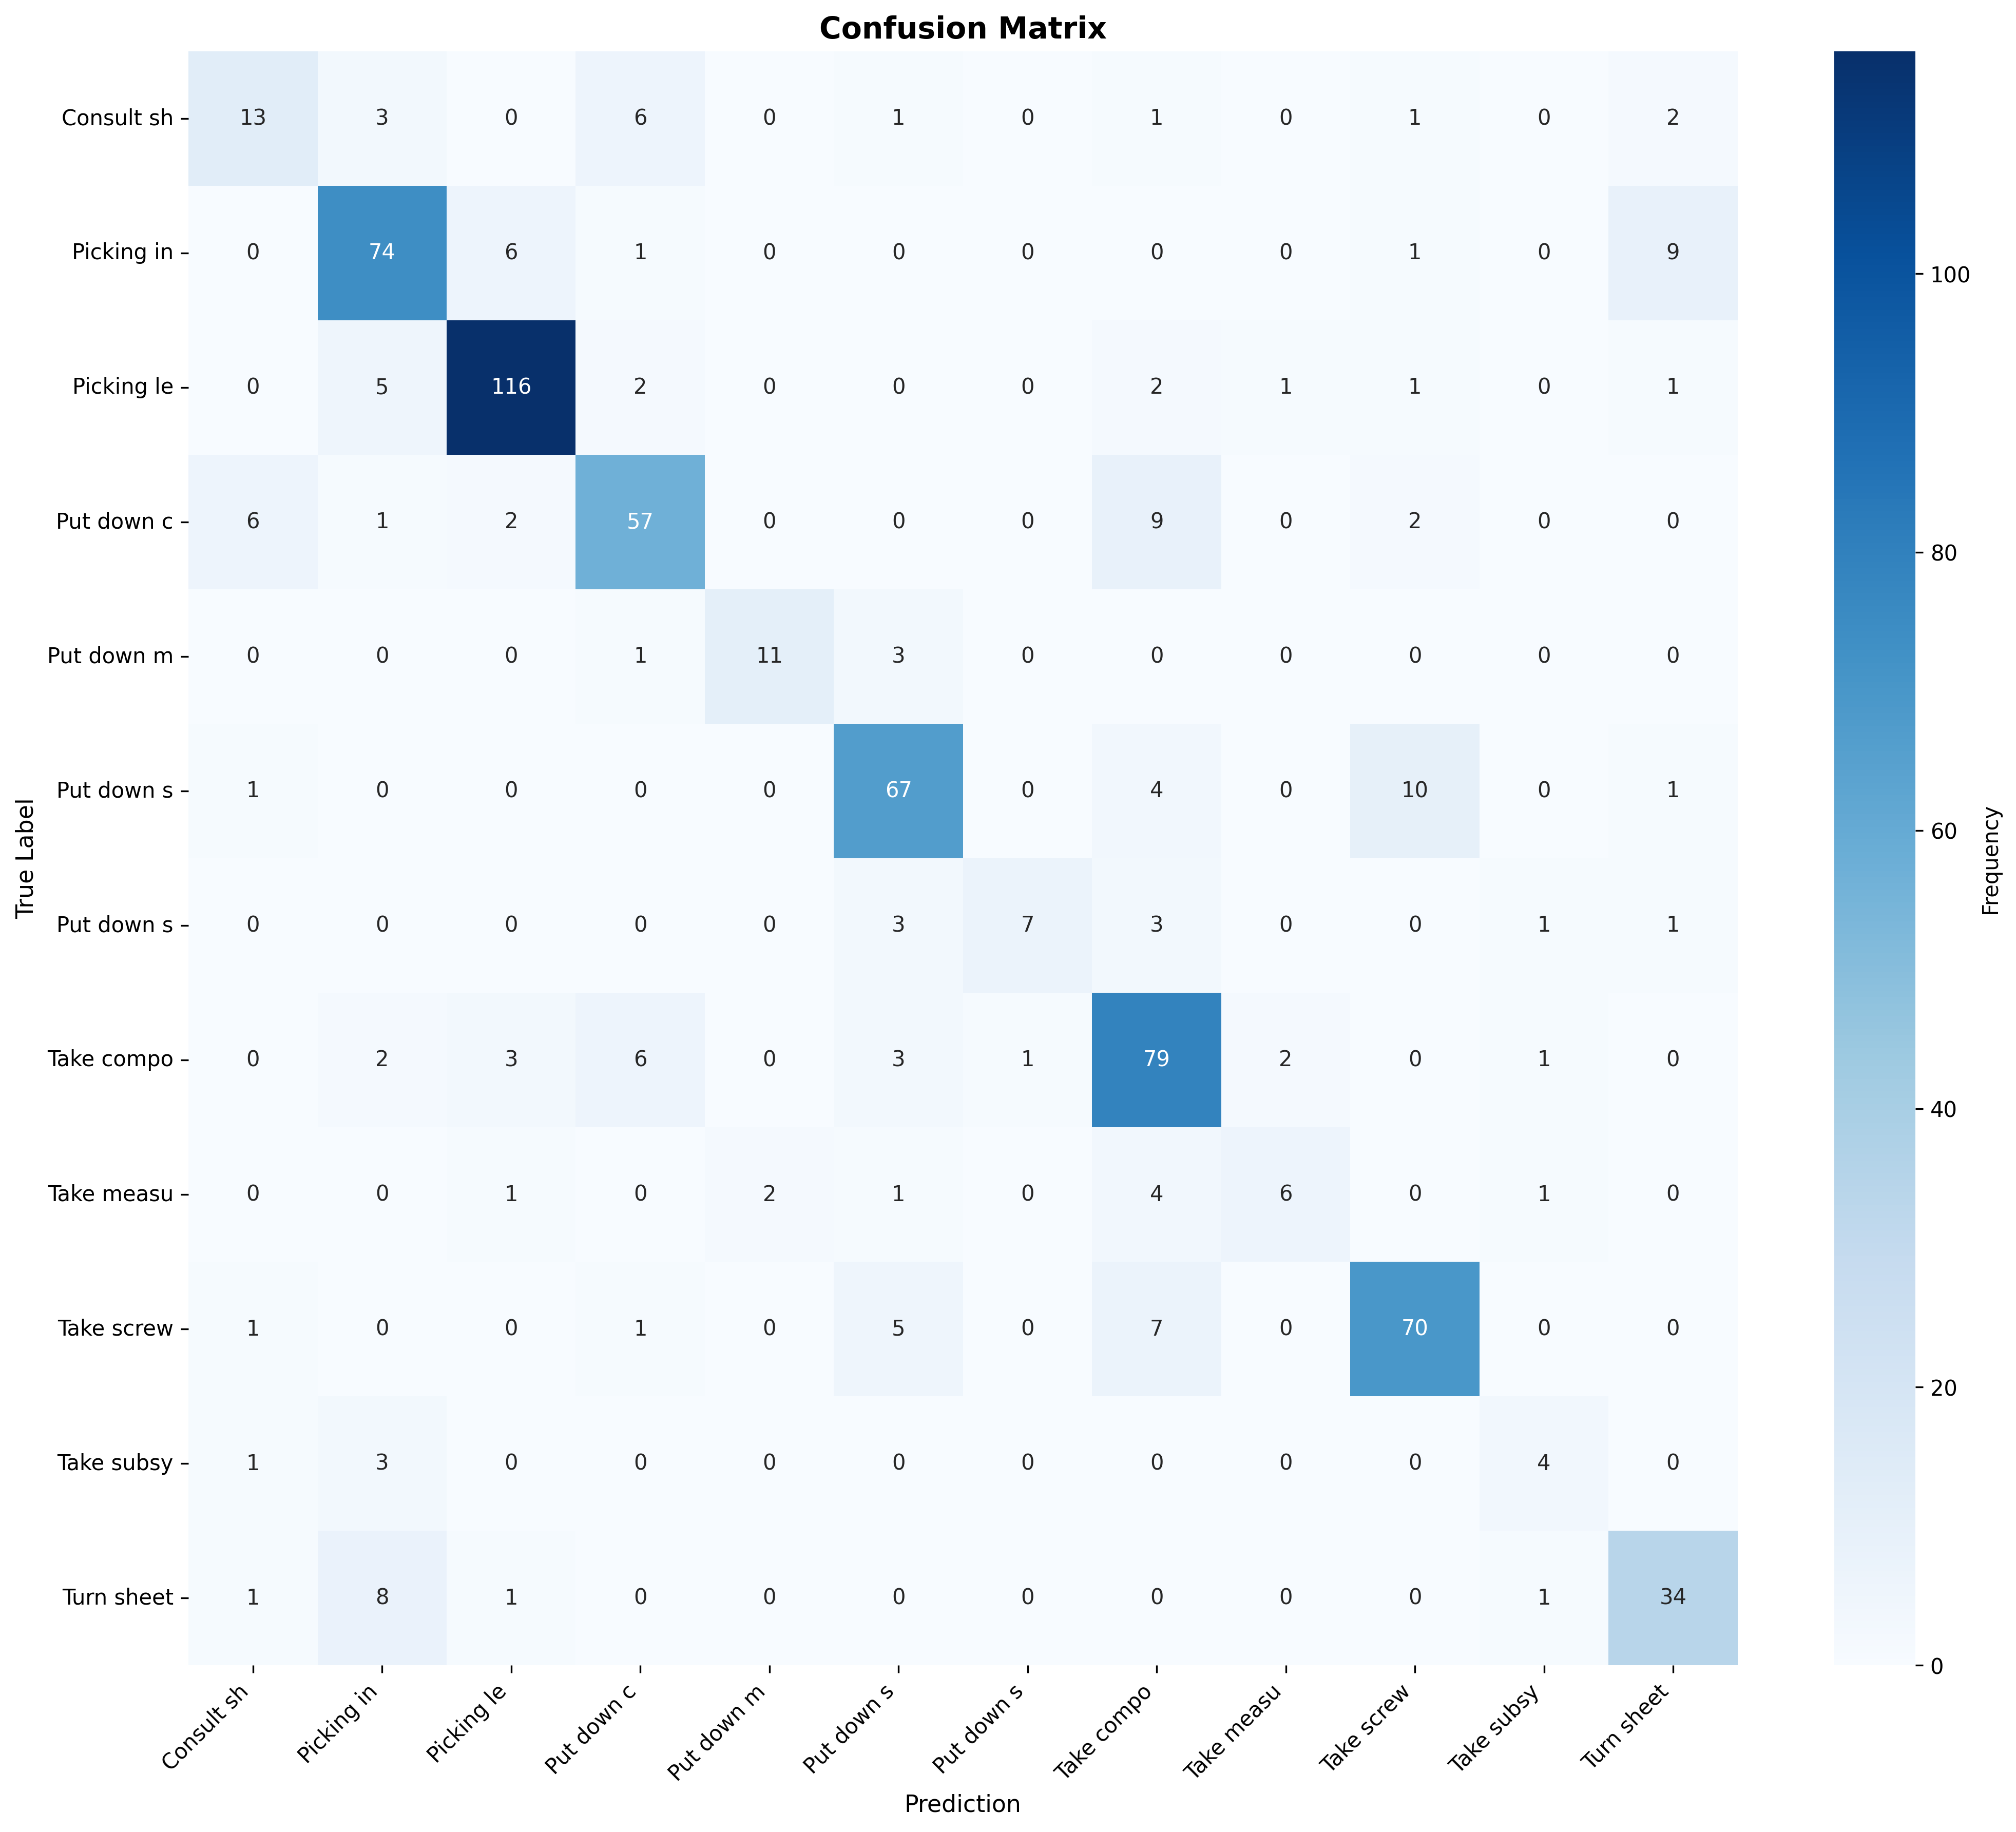
\includegraphics[width=0.95\textwidth]{01_confusion_matrix.png}
\caption{Matriz 12×12 del modelo V-JEPA 2. Diagonal fuerte indica alta precisión (78.54\%). Algunas confusiones entre clases similares (ej: picking left vs picking front).}
\label{fig:cm}
\end{figure}

\subsection{Gráfico 2: Métricas por Clase}

\begin{figure}[H]
\centering
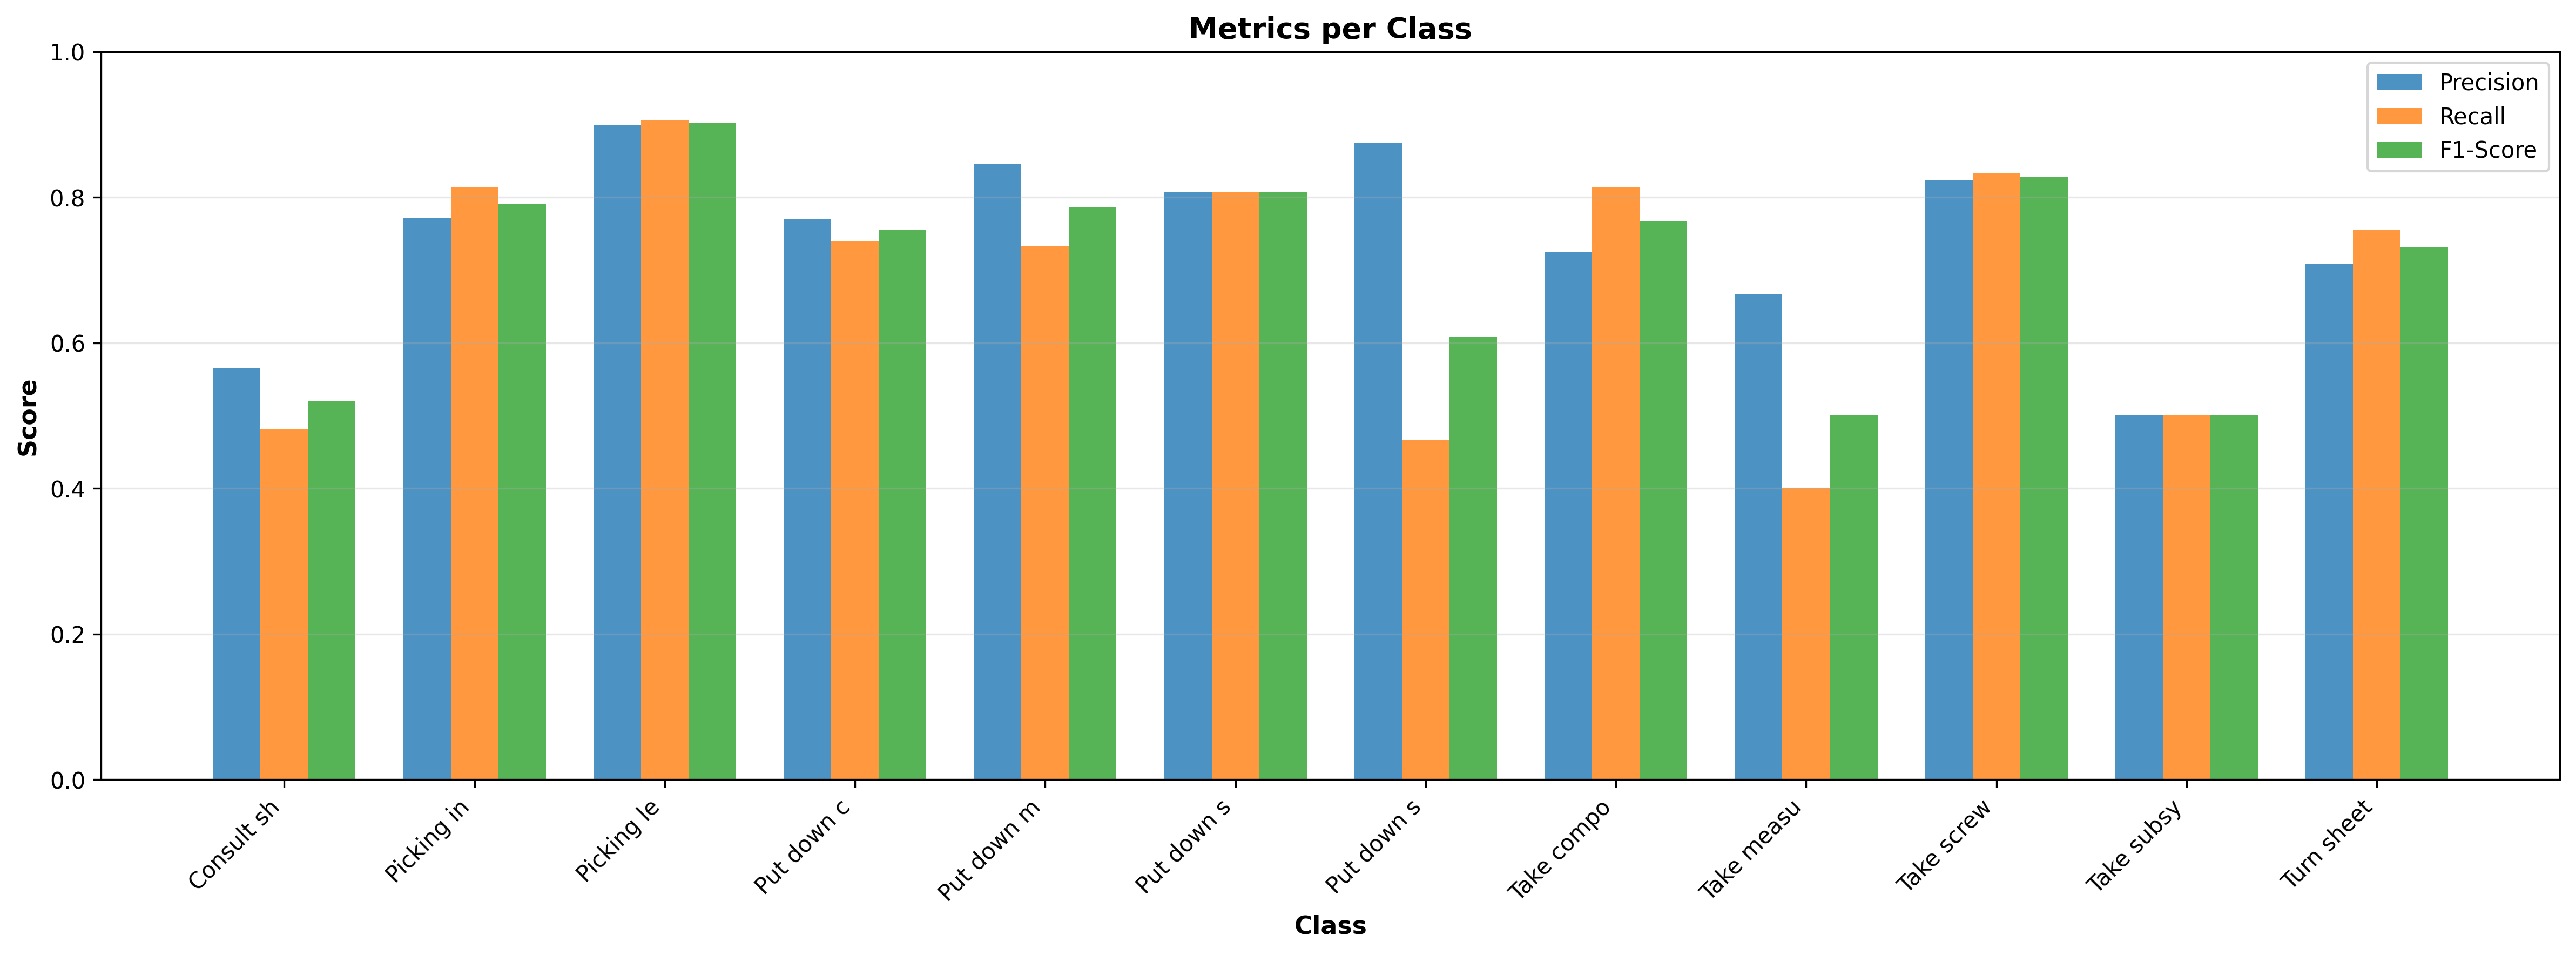
\includegraphics[width=0.95\textwidth]{02_metrics_per_class.png}
\caption{Precision, Recall, F1-score por acción. Mayoría de clases F1 > 0.65. Clases con pocos ejemplos tienen rendimiento más variable.}
\label{fig:metrics}
\end{figure}

\subsection{Gráfico 3: Curvas ROC (One-vs-Rest)}

\begin{figure}[H]
\centering
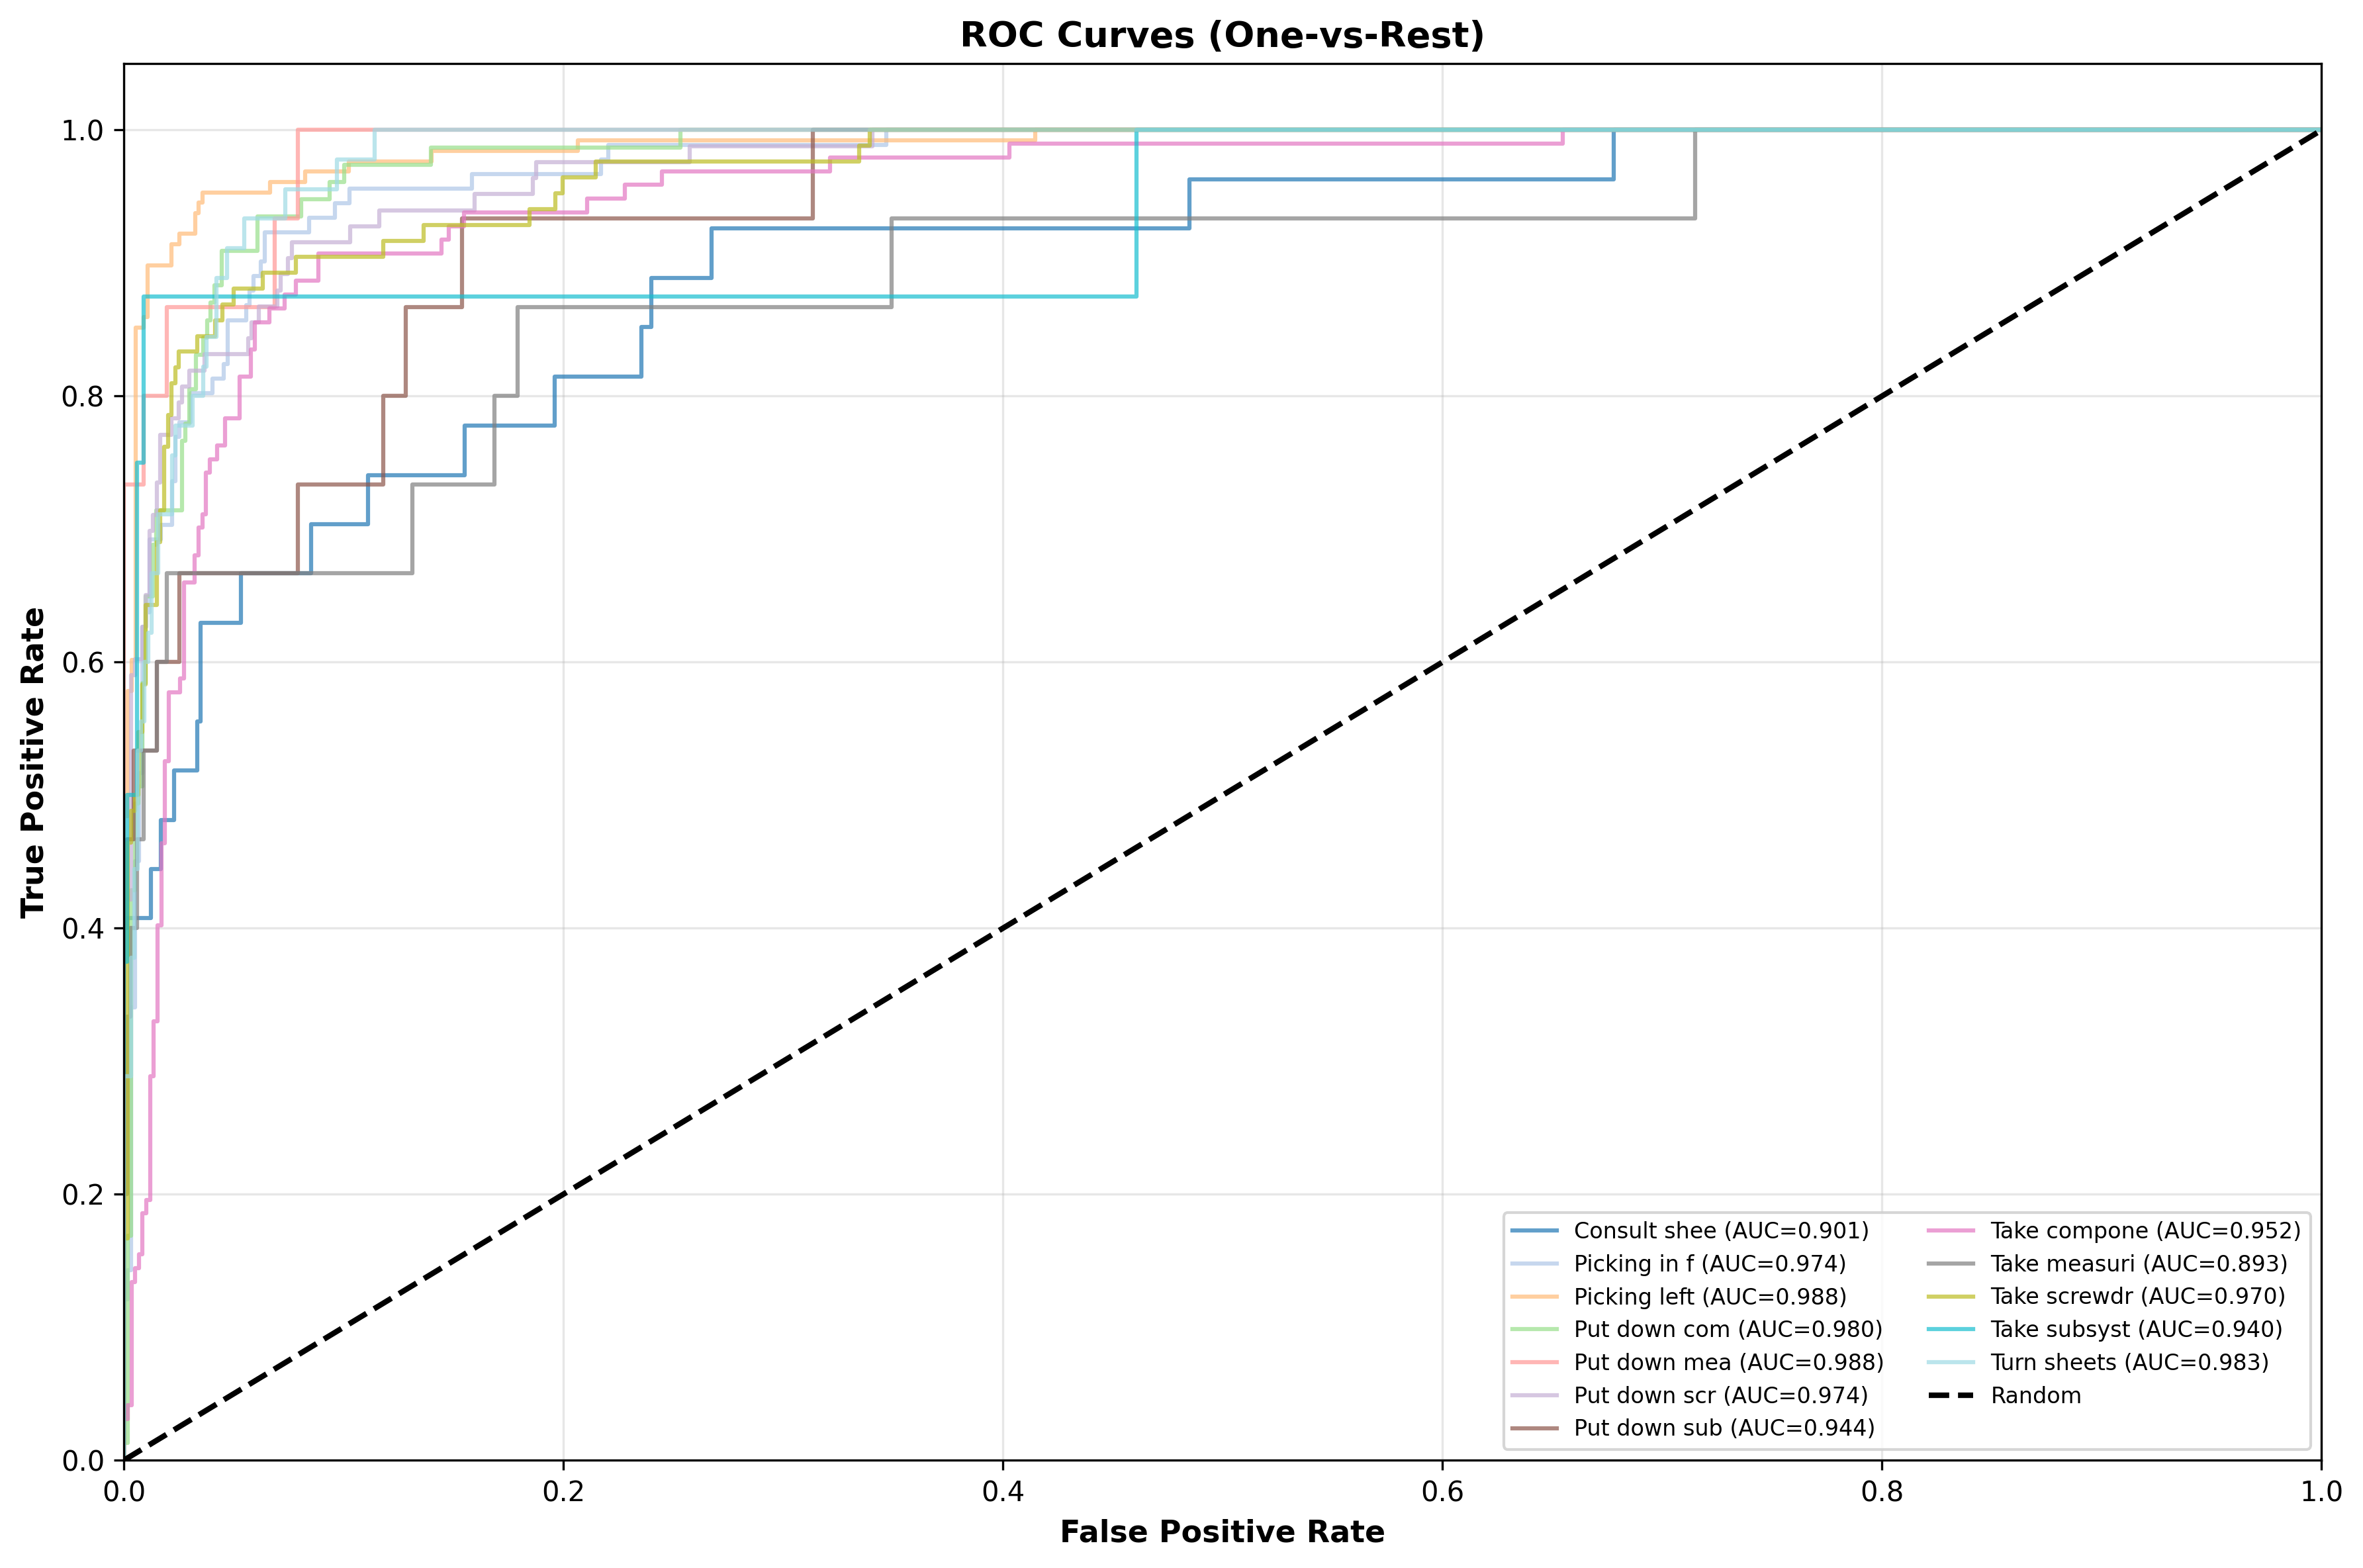
\includegraphics[width=0.95\textwidth]{03_roc_curve.png}
\caption{12 curvas ROC (una por clase). Mean AUC = 0.9573 (Excelente discriminación). Todas las curvas cercanas a esquina superior izquierda.}
\label{fig:roc}
\end{figure}

\subsection{Gráfico 4: Distribución de Confianza}

\begin{figure}[H]
\centering
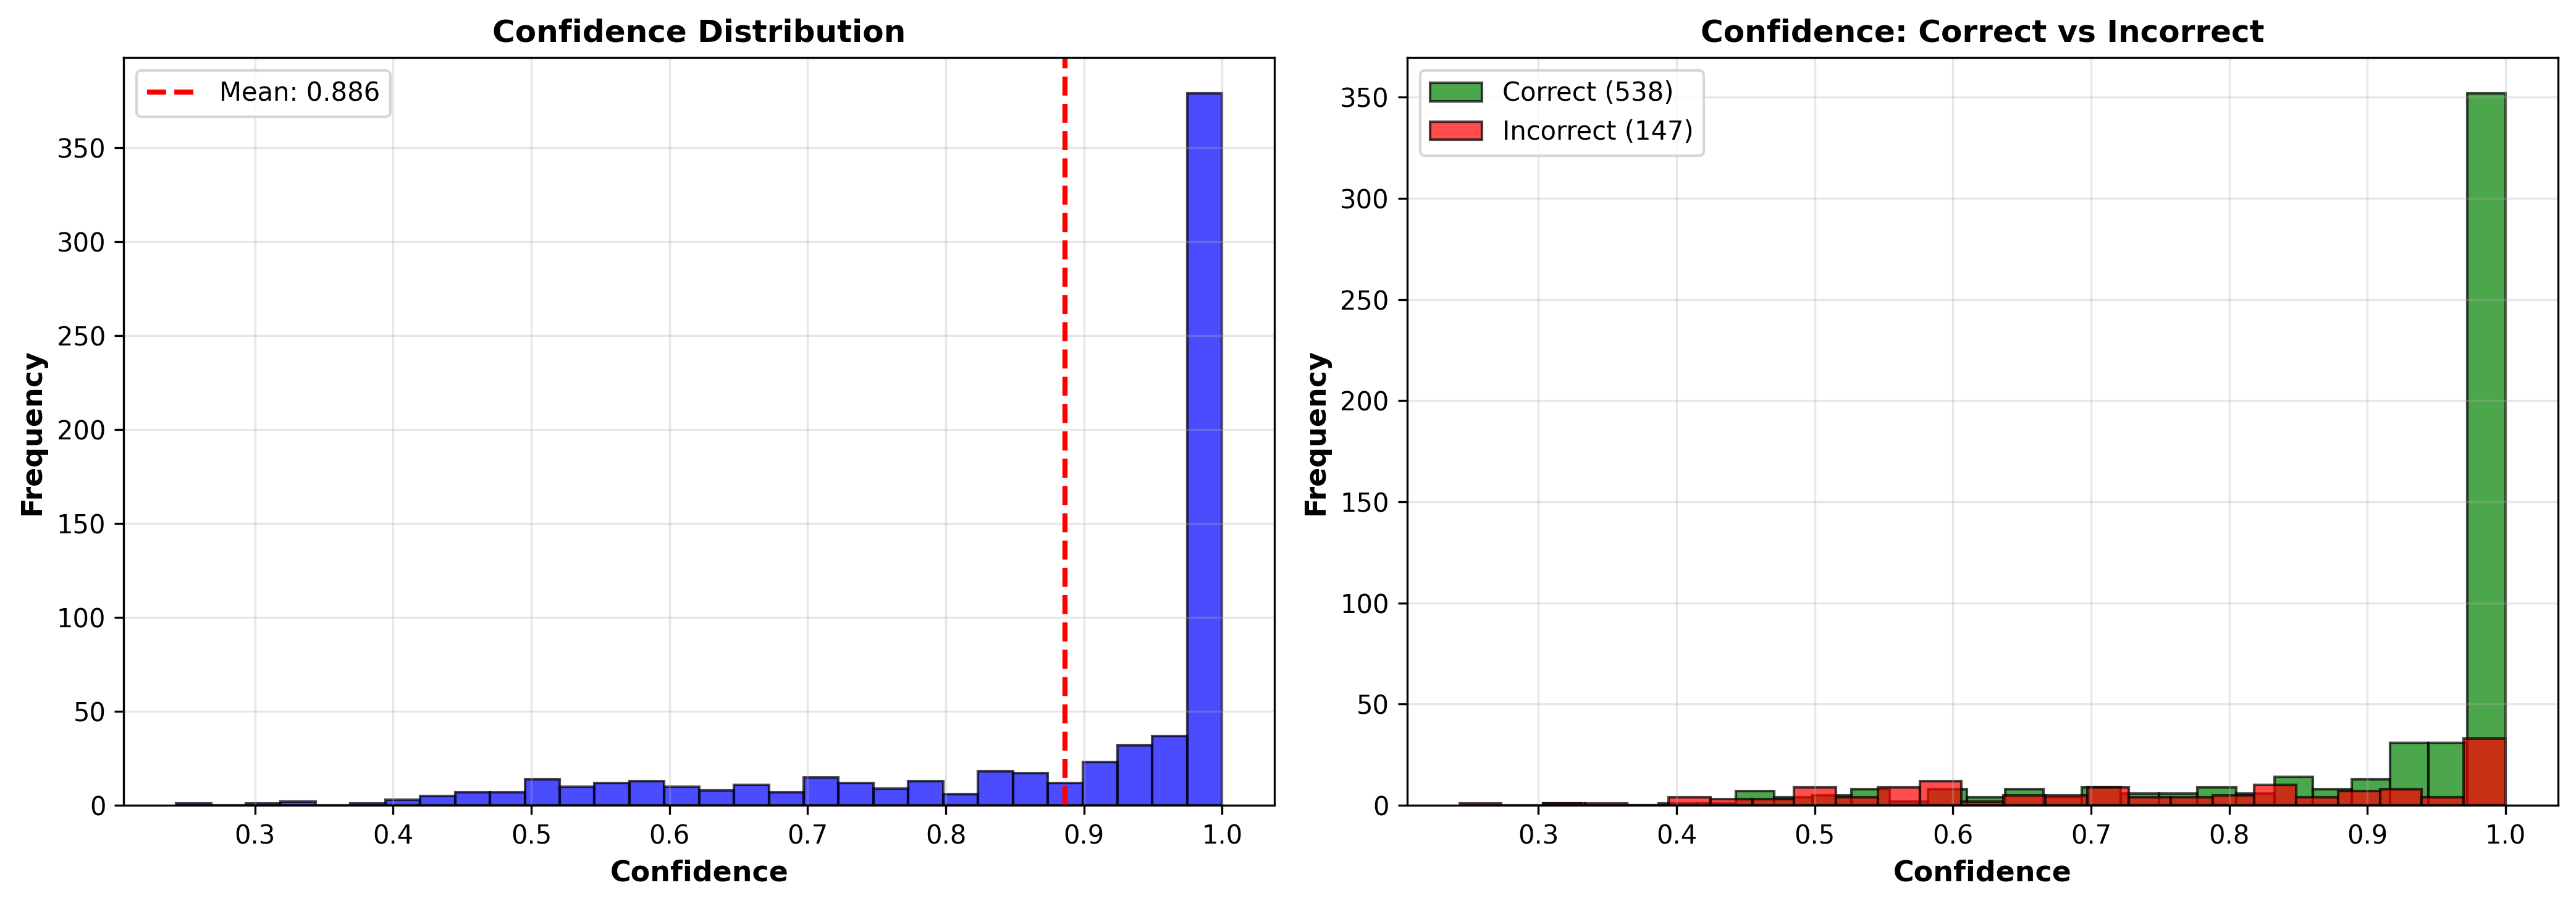
\includegraphics[width=0.95\textwidth]{04_confidence_distribution.png}
\caption{Confianza promedio 0.85. Buena separación entre predicciones correctas (confianza mayor) e incorrectas. Modelo bien calibrado.}
\label{fig:conf}
\end{figure}

\subsection{Gráfico 5: Balance de Clases vs Accuracy}

\begin{figure}[H]
\centering
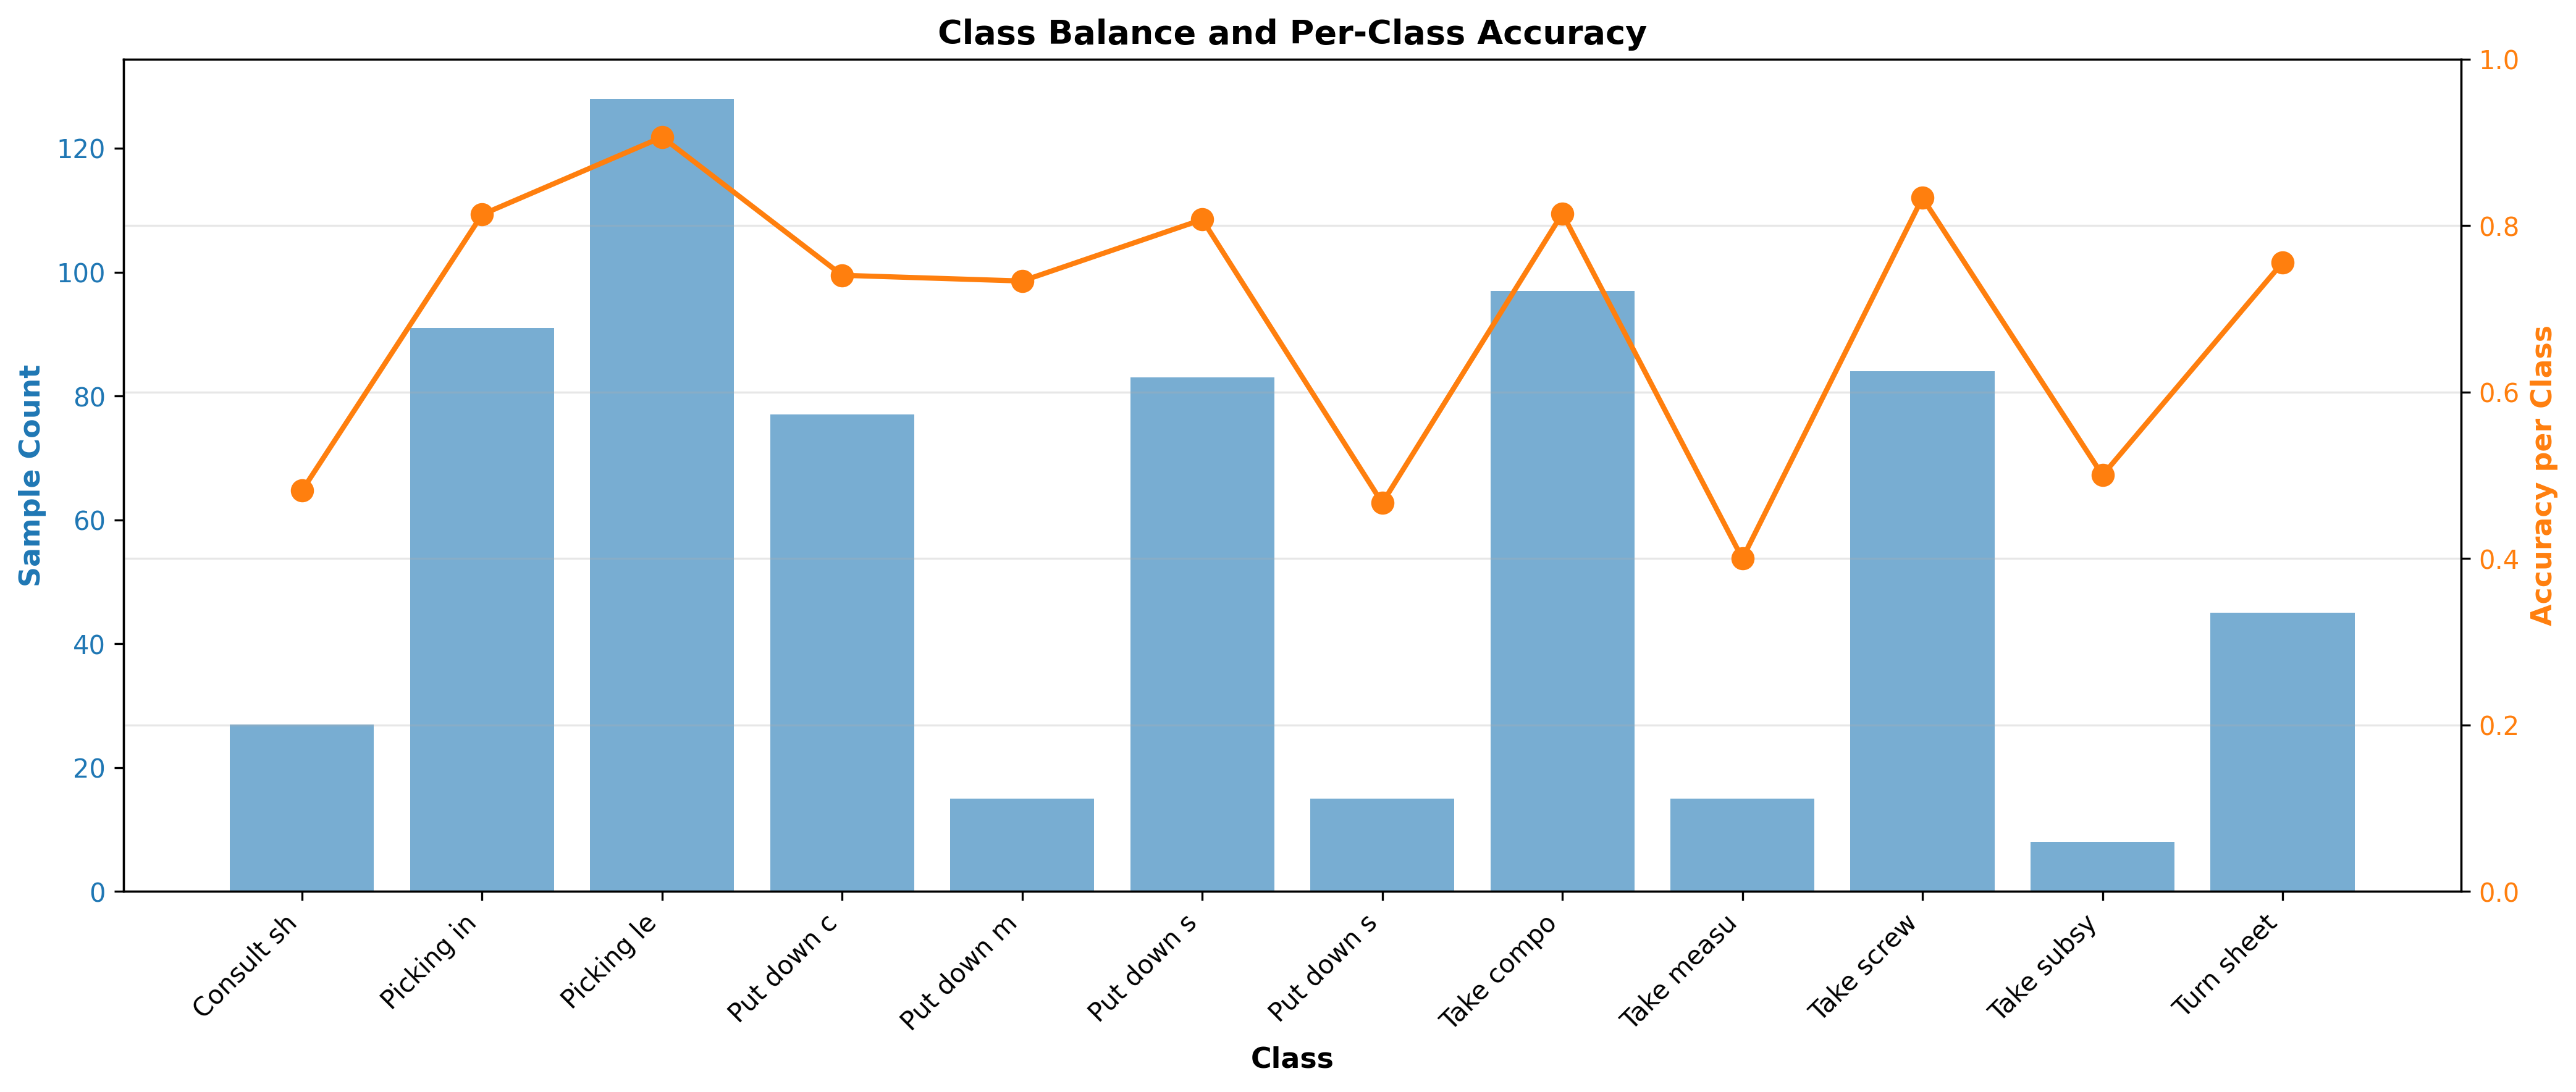
\includegraphics[width=0.95\textwidth]{05_class_balance_and_accuracy.png}
\caption{Correlación inversa: clases con pocos ejemplos tienen menor accuracy. Oportunidad: aumentar datos de clases minoritarias.}
\label{fig:balance}
\end{figure}

\section{Análisis y Hallazgos}

\begin{itemize}
  \item \textbf{Modelos Base:} V-JEPA 2 superior (78.54\%). DINOv2 competitivo pero menor accuracy.
  \item \textbf{Ensambles Heterogéneos:} No mejoran sobre base. Stacking 75.80\%, Blending 74.84\%.
  \item \textbf{Ensambles Homogéneos:} Degradación severa (51-40\%). Los embeddings pre-entrenados congelados no se benefician de promediación.
  \item \textbf{Discriminación:} AUC 0.9573 indica excelente separación de clases.
  \item \textbf{Calibración:} Confianza 0.85 correlaciona bien con acierto.
\end{itemize}

\section{Modelo Final Seleccionado}

\textbf{V-JEPA 2} es el ganador entre 7 modelos evaluados.

\textbf{Especificación:}
\begin{itemize}
  \item Backbone: Vision Joint Embedding Predictive Architecture v2
  \item Embeddings: 1024 dims (congelados)
  \item Clasificador: Regresión Logística (12 clases)
  \item Latencia: <5ms (tiempo real)
\end{itemize}

\textbf{Performance:}
\begin{itemize}
  \item Accuracy: 78.54\%
  \item Macro F1: 0.7063
  \item AUC-ROC: 0.9573 (Excelente)
  \item Confianza promedio: 0.85
\end{itemize}

\textbf{Justificación:} Máxima accuracy, excelente discriminación (AUC 0.9573), eficiencia temporal, buena calibración, escalable a nuevas acciones.

\section{Recomendaciones}

\begin{enumerate}
  \item \textbf{Despliegue inmediato:} Integrar V-JEPA 2 en vision-ops-backend con threshold confianza 0.75
  \item \textbf{Validación HITL:} Registrar predicciones en SQLite, validación en producción
  \item \textbf{Mejora continua:} Recolectar datos reales, fine-tuning selectivo, aumentar clases minoritarias (SMOTE)
  \item \textbf{Benchmarking:} Comparar contra operadores humanos
\end{enumerate}

\section{Conclusión}

Se completó exitosamente el análisis de 7 modelos (2 base + 5 ensambles). V-JEPA 2 es el ganador con 78.54\% accuracy y AUC 0.9573. El modelo base pre-entrenado es más efectivo que las estrategias de ensamble evaluadas. Está listo para despliegue en producción.

\end{document}
